% ef research
% ch 2, 4, 5

\section{Energy forecasting research}


\subsection{Probabilistic scores}
\begin{frame}{Pinball loss}
    The pinball score or quantile score is used to measure the accuracy of a quantile forecast.
\begin{definition}
    The pinball loss is defined as
    $$
    \mathrm{Pinball}(y_{t},\hat{y}_{t,q},q)=
\begin{cases}
(q-1)(\hat{y}_{t,q}-y_{t}) & y_t > \hat{y}_{t,q} \\
q(\hat{y}_{t,q}-y_t) & y_t \leq \hat{y}_{t,q}
\end{cases}
$$
\end{definition}
\end{frame}


\begin{frame}{Pinball loss}
    The pinball loss is an asymmetric function, it weights its score differently depending on the error sign and on the quantile considered.
By averaging all the pinball losses over all quantiles and over the whole forecast horizon, we obtain the pinball loss of the probabilistic forecast.
    \begin{center}
        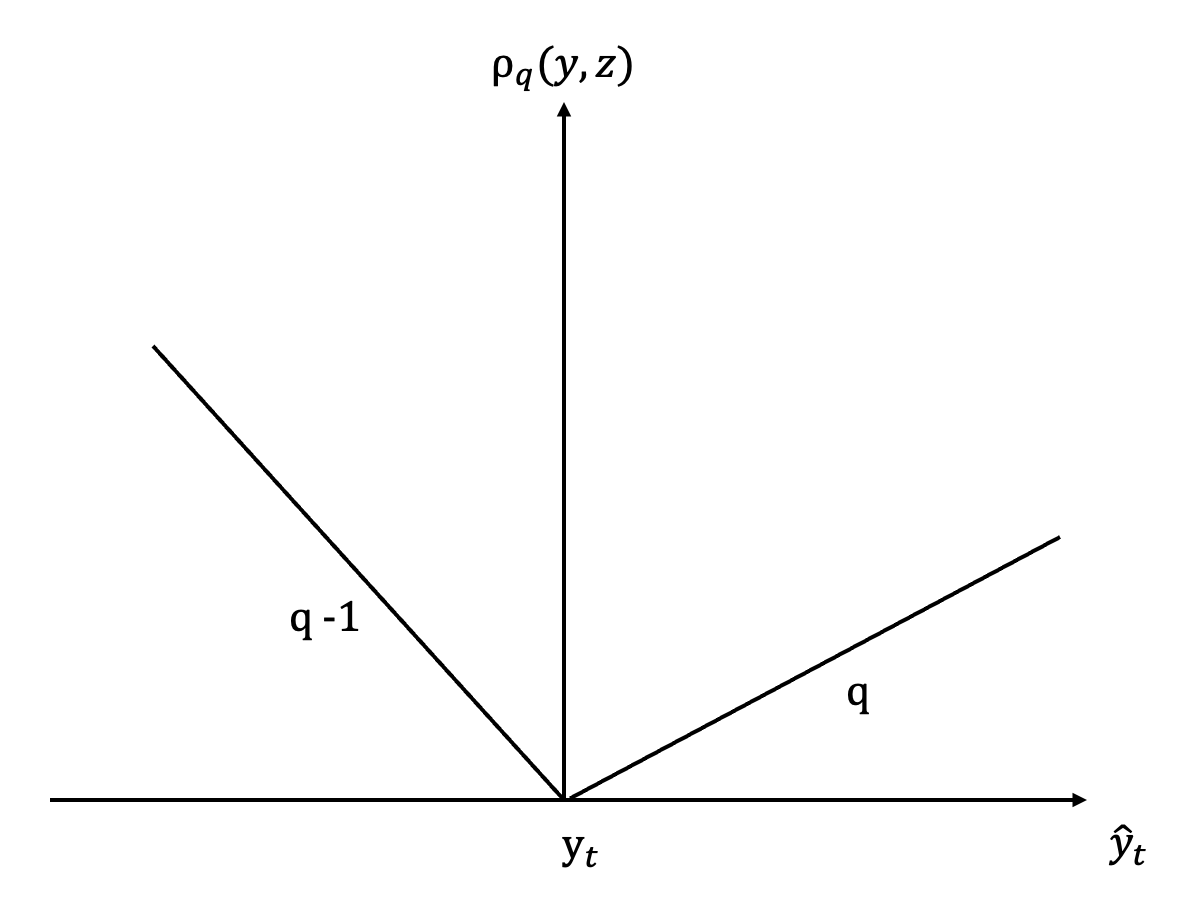
\includegraphics[height=0.5\textheight]{../thesis/images/pinball_loss.png}
    \end{center}
\end{frame}





\begin{frame}{Continous ranked probability score}
The continous ranked probability score (CRPS) measures the difference between the estimated cumulative distribution $\hat{F}$ and the empirical cumulative density function (CDF).
\begin{definition}\label{def_crps}
    The continous ranked probability score is defined as
    $$
    \mathrm{CRPS}(y, \hat{F})=\int\limits_{-\infty}^{\infty}\left(\hat{F}(x)-\mathbb{I}_{\{x-y\}} \right)^2 dx
    $$
\end{definition}
% Nevertheless, we can evaluate the integral in closed form. 
Where the indicator function is defined as 
    $$\mathbb{I}_{\{z\}}=
\begin{cases}
0, & z<0\\
1, & z \geq 0
\end{cases}$$
\end{frame}


\begin{frame}{Continous ranked probability score}
    For a visualisation see Figure. The grey area is what contributes toward the CRPS score.
    The better the estimated cumulative density function is the smaller the total CRPS score will be.
    \begin{figure}
        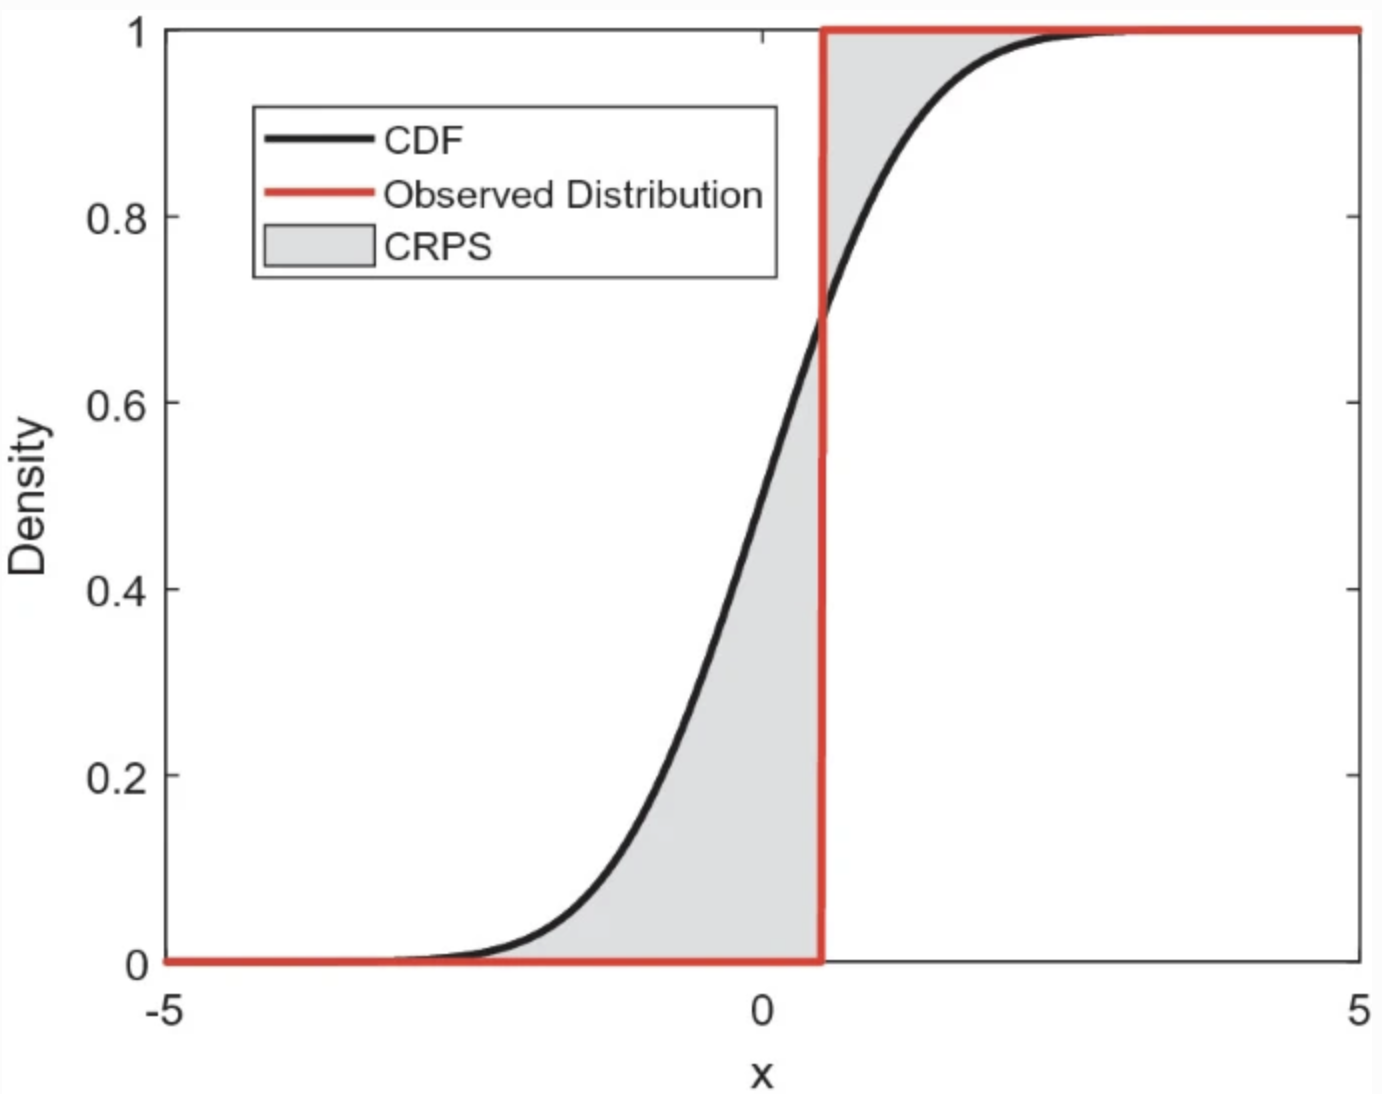
\includegraphics[width=0.5\textwidth]{../thesis/images/crps.png}
    \end{figure}
\end{frame}